\chapter{Технологический раздел}
\label{cha:impl}

В данном разделе будут составлены требования к программному обеспечению, выбраны средства реализации и определены тестовые данные.

\section{Требования к программному обеспечению}
Требования к вводу:
\begin{itemize}
    \item размер массива;
    \item элементы массива, разделенные произвольным количеством пробельных символов.
\end{itemize}

Требования к выводу:
\begin{itemize}
    \item отсортированный массив.
\end{itemize}

Требования к программе:
\begin{itemize}
    \item выбор алгоритма происходит через аргументы командной строки путём передачи его номера:
        \begin{enumerate}[1)]
            \item быстрая сортировка;
            \item сортировка вставками;
            \item шейкерная сортировка.
        \end{enumerate}

\end{itemize}

\section{Средства реализации}
Для реализации программы вычисления редакционного расстояния мной был выбран язык программирования C++. В рамках текущей задачи данный язык программирования имеет ряд существенных преимуществ:
\begin{itemize}
    \item Статическая типизация;
    \item Близость к низкоуровневому C при наличии многих возможностейвысоко уровненных языков;
    \item Встроенная библиотека std::chrono, позволяющая измерять процессорное время \cite{chrono}.
\end{itemize}

\section{Листинги кода}

В листингах \ref{lst:qs}, \ref{lst:ins}, \ref{lst:shs} приведены текста функций быстрой сортировки, сортировки вставками и шейкерной сортировки соответственно.

\noindent\begin{minipage}{\textwidth}
\begin{lstlisting}[caption=Сортировка вставками, label=lst:ins]
#define swp(val1, val2) { auto tmp = val1; val1 = val2; val2 = tmp; }

template <typename Type>
void insertionsort(Type *arr, int len, bool (*comp)(Type, Type))
{
    for (int i = 1; i < len; i++)
    {
        for (int j = i; j > 0 && comp(arr[j - 1], arr[j]); j--)
        {
            swp(arr[j], arr[j - 1]);
        }
    }
}

#undef swp
\end{lstlisting}
\end{minipage}

\noindent\begin{minipage}{\textwidth}
\begin{lstlisting}[caption=Бастрая сортировка, label=lst:qs]
#define swp(val1, val2) { auto tmp = val1; val1 = val2; val2 = tmp; }

template <typename Type>
static int parition(Type *arr, int low, int high, bool (*comp)(Type, Type))
{
    int i = low;
    Type pivot = arr[high];

    for (int j = low; j < high; j++)
    {
        if (comp(pivot, arr[j]))
        {
            swp(arr[i], arr[j]);
            i++;
        }
    }

    swp(arr[i], arr[high]);

    return i;
}

template <typename Type>
static void qsrec(Type *arr, int low, int high, bool (*comp)(Type, Type))
{
    if (low < high)
    {
        int p = parition(arr, low, high, comp);

        qsrec(arr, low, p - 1, comp);
        qsrec(arr, p + 1, high, comp);
    }
}

template <typename Type>
void quicksort(Type *arr, int len, bool (*comp)(Type, Type))
{
    qsrec(arr, 0, len - 1, comp);
}

#undef swp
\end{lstlisting}
\end{minipage}

\noindent\begin{minipage}{\textwidth}
\begin{lstlisting}[caption=Шейкреная сортировка, label=lst:shs]
#define swp(val1, val2) { auto tmp = val1; val1 = val2; val2 = tmp; }

template <typename Type>
void shakersort(Type *arr, int len, bool (*comp)(Type, Type))
{
    int low = 0;
    int high = len - 1;

    while (low <= high)
    {
        for (int idx = low; idx < high; idx++)
        {
            if (comp(arr[idx], arr[idx + 1]))
            {
                swp(arr[idx], arr[idx + 1]);
            }
        }
        high--;

        for (int idx = high; idx > low; idx--)
        {
            if (comp(arr[idx - 1], arr[idx]))
            {
                swp(arr[idx], arr[idx - 1]);
            }
        }
        low++;
    }
}

#undef swp
\end{lstlisting}
\end{minipage}

\section{Примеры работы}

На рисунках \ref{img:notfullinput}-\ref{img:similar} приведены примеры работы реализованной программы.

\begin{figure}[H]
    \centering
    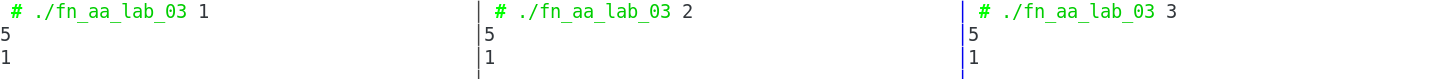
\includegraphics[scale=0.5]{./images/example01.png}
    \caption{Преждевременное завершение ввода}
    \label{img:notfullinput}
\end{figure}
\begin{figure}[H]
    \centering
    
\includegraphics[scale=0.5]{./images/example02.png}
    \caption{Пустой ввод}
    \label{img:emptyinput}
\end{figure}
\begin{figure}[H]
    \centering
    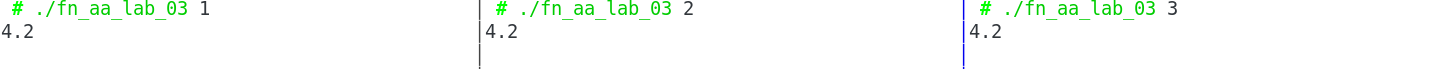
\includegraphics[scale=0.5]{./images/example03.png}
    \caption{Некорректный ввод}
    \label{img:wronginput}
\end{figure}
\begin{figure}[H]
    \centering
    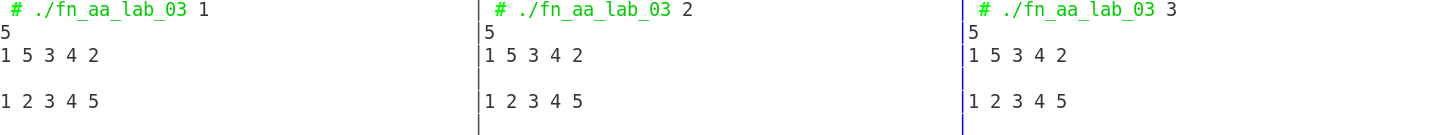
\includegraphics[scale=0.5]{./images/example04.png}
    \caption{Массив произвольной степени сортированности}
    \label{img:notsorted}
\end{figure}
\begin{figure}[H]
    \centering
    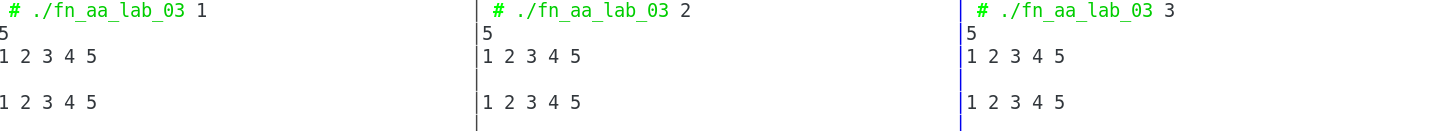
\includegraphics[scale=0.5]{./images/example05.png}
    \caption{Отсортированный массив}
    \label{img:sorted}
\end{figure}
\begin{figure}[H]
    \centering
    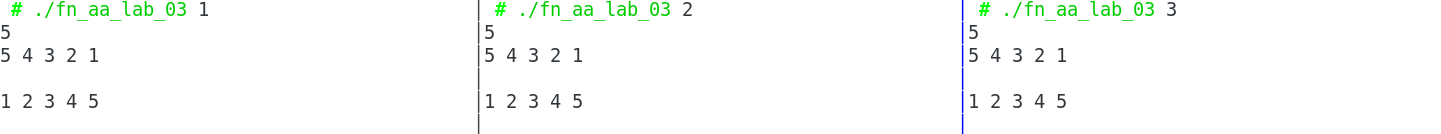
\includegraphics[scale=0.5]{./images/example06.png}
    \caption{Обратно отсортированный массив}
    \label{img:reversed}
\end{figure}
\begin{figure}[H]
    \centering
    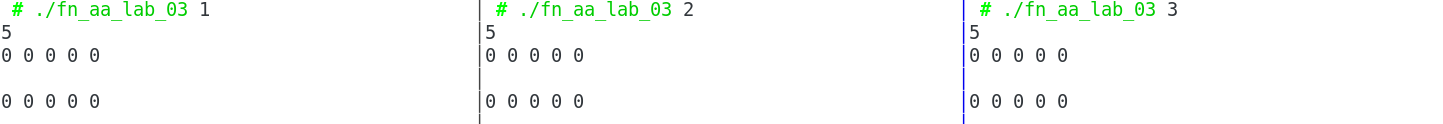
\includegraphics[scale=0.5]{./images/example07.png}
    \caption{Массив из одинаковых чисел}
    \label{img:similar}
\end{figure}


\section{Описание тестирования}
Для тестирования программы были подготовлены тестовые данные, указанные в таблице \ref{table:test}.

\begin{table}[H]
    \centering
    \caption{Тестовые данные}
    \label{table:test}
    \begin{tabular}{|c|c|}
        \hline
        Входной массив & Ожидаемый результат \\
        \hline
        1, 2, 3, 4, 5, 6, 7, 8, 9 & 1, 2, 3, 4, 5, 6, 7, 8, 9 \\
        \hline
        9, 8, 7, 6, 5, 4, 3, 2, 1 & 1, 2, 3, 4, 5, 6, 7, 8, 9 \\
        \hline
        4, 2, 7, 4, 8, 2, 4, 8, 1 & 1, 2, 2, 4, 4, 4, 7, 8, 8 \\
        \hline
        5, 5, 5, 5, 5, 5, 5, 5, 5 & 5, 5, 5, 5, 5, 5, 5, 5, 5 \\
        \hline
    \end{tabular}
\end{table}

Результаты тестирования приведены в таблицах \ref{table:qsres}, \ref{table:inres}, \ref{table:shres}. Все тесты были успешно пройдены.

\begin{table}[H]
    \centering
    \caption{Результаты тестирования быстрой сортировки}
    \label{table:qsres}
    \begin{tabular}{|c|c|}
        \hline
        Входной массив & Результат \\
        \hline
        1, 2, 3, 4, 5, 6, 7, 8, 9 & 1, 2, 3, 4, 5, 6, 7, 8, 9 \\
        \hline
        9, 8, 7, 6, 5, 4, 3, 2, 1 & 1, 2, 3, 4, 5, 6, 7, 8, 9 \\
        \hline
        4, 2, 7, 4, 8, 2, 4, 8, 1 & 1, 2, 2, 4, 4, 4, 7, 8, 8 \\
        \hline
        5, 5, 5, 5, 5, 5, 5, 5, 5 & 5, 5, 5, 5, 5, 5, 5, 5, 5 \\
        \hline
    \end{tabular}
\end{table}

\begin{table}[H]
    \centering
    \caption{Результаты тестирования сортировки вставками}
    \label{table:inres}
    \begin{tabular}{|c|c|}
        \hline
        Входной массив & Результат \\
        \hline
        1, 2, 3, 4, 5, 6, 7, 8, 9 & 1, 2, 3, 4, 5, 6, 7, 8, 9 \\
        \hline
        9, 8, 7, 6, 5, 4, 3, 2, 1 & 1, 2, 3, 4, 5, 6, 7, 8, 9 \\
        \hline
        4, 2, 7, 4, 8, 2, 4, 8, 1 & 1, 2, 2, 4, 4, 4, 7, 8, 8 \\
        \hline
        5, 5, 5, 5, 5, 5, 5, 5, 5 & 5, 5, 5, 5, 5, 5, 5, 5, 5 \\
        \hline
    \end{tabular}
\end{table}

\begin{table}[H]
    \centering
    \caption{Результаты тестирования шейкреной сортировки}
    \label{table:shres}
    \begin{tabular}{|c|c|}
        \hline
        Входной массив & Результат \\
        \hline
        1, 2, 3, 4, 5, 6, 7, 8, 9 & 1, 2, 3, 4, 5, 6, 7, 8, 9 \\
        \hline
        9, 8, 7, 6, 5, 4, 3, 2, 1 & 1, 2, 3, 4, 5, 6, 7, 8, 9 \\
        \hline
        4, 2, 7, 4, 8, 2, 4, 8, 1 & 1, 2, 2, 4, 4, 4, 7, 8, 8 \\
        \hline
        5, 5, 5, 5, 5, 5, 5, 5, 5 & 5, 5, 5, 5, 5, 5, 5, 5, 5 \\
        \hline
    \end{tabular}
\end{table}


\section{Вывод}
Таким образом, были сформулированы требования к реализуемой программе, выбран язык программирования C++ в качестве основного инструмента разработки, и успешно проведены тесты, подтверждающие правильность работы разработанной программы.

